\section{Direct products and direct sums}
\begin{ex}
    $S_{3}$ is not the direct product of any family of its proper subgroups. The same is true of $Z_{p^{n}}$($p$ prime, $n\geq 1$) and $\mathbb{Z}$.
\end{ex}

$$ $$

\begin{ex}
    Give an example of groups $H_{i}$, $K_{i}$ such that $H_{1}\times H_{2}\cong K_{1}\times K_{2}$ and no $H_{i}$ is isomorphic to any $K_{j}$.
\end{ex}

$$ $$

\begin{ex}
    Let $G$ be and (additive) abelian group with subgroups $H$ and $K$. Show that $G\cong H\oplus K$ if and only if there are homomorphisms 
    
    \begin{figure}[H]\centering
        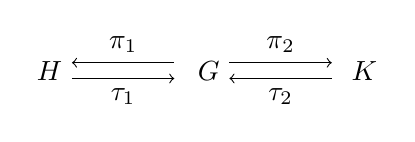
\begin{tikzpicture}
            \node [left] at (0,1) {$H$};
            \node [left] at (2,1) {$G$};
            \node [left] at (4,1) {$K$};
            \draw [<-] (0,1.1)-- node [above, pos=0.5]{$\pi_{1}$} (1.3,1.1);
            \draw [->] (0,0.9)-- node [below, pos=0.5]{$\tau_{1}$} (1.3,0.9);
            \draw [->] (2,1.1)-- node [above, pos=0.5]{$\pi_{2}$} (3.3,1.1);
            \draw [<-] (2,0.9)-- node [below, pos=0.5]{$\tau_{2}$} (3.3,0.9);
        \end{tikzpicture}
    \end{figure}
    such that $\pi_{1}\tau_{1}=1_{H}$, $\pi_{2}\tau_{2}=1_{K}$, $\pi_{1}\tau_{2}=0$ and $\pi_{2}\tau_{1}=0$, where 0 is the map sending every element onto the zero (identity) element, and $\tau_{1}\pi_{1}(x)+\tau_{2}\pi_{2}(x)=x$ for all $x\in G$.
\end{ex}

$$ $$

\begin{ex}
    Give an example to show that the weak direct product is not a coproduct in the category of all groups.
\end{ex}

$$ $$

\begin{ex}
    Let $G$, $H$ be finite cyclic groups. Then $G\times H$ is cyclic if and only if $(\left| G \right|, \left| H \right|  )=1$.
\end{ex}

$$ $$

\begin{ex}
    Every finitely generated abelian group $G\neq\left\langle e\right\rangle$ in which every element (except $e$) has order $p$ ($p$ prime) is isomorphic to $Z_{p}\oplus Z_{p}\oplus\cdots\oplus Z_{p}$($n$ summands) for some $n\geq 1$.
\end{ex}

$$ $$

\begin{ex}
    Let $H,K,N$ be nontrivial normal subgroups of a group $G$ and suppose $G=H\times K$. Prove that $N$ is in the center of $G$ or $N$ intersects one of $H,K$ nontrivially. Give examples to show that both possibilities can actually occur when $G$ is nonabelian.
\end{ex}

$$ $$

\begin{ex}
    Corollary 8.7 is false if one of the $N_{i}$ is not normal.
\end{ex}

$$ $$

\begin{ex}
    If a group $G$ is the (internal) direct product of its subgroups $H$, $K$, then $H\cong G / K$ and $G /H \cong K$.
\end{ex}

$$ $$

\begin{ex}
    If $\{G_{i}|i\in I\}$ is a family of groups, then $\prod^{w}G_{i}$ is the internal weak product its subgroups $\{\tau_{i}(G_{i})|i\in I\}$.
\end{ex}

$$ $$

\begin{ex}
    Let $\{N_{i}|i\in I\}$ be a family of subgroups of a group $G$. Then $G$ is the internal weak product of $\{N_{i}|i\in I\}$if and only if:
    \begin{enumerate}[(i)]
        \item $a_{i}a_{j}=a_{j}a_{i}$ for all $i\neq j$ and $a_{i}\in N_{i}$, $a_{j}\in N_{j}$;
        \item every nonidentity element of $G$ is uniquely a product $a_{i_{1}}\cdots a_{i_{n}}$, where $i_{i},\dots,i_{n}$ are distinct elements of $I$ and $e\neq a_{i_{k}}\in N_{i_{k}}$ for each $k$.
    \end{enumerate}
\end{ex}

$$ $$

\begin{ex}
    A normal subgroup $H$ of a group $G$ is said to be a \textbf{direct factor} (\textbf{direct summand} if $G$ is additive abelian) if there exists a (normal) subgroup $K$ of $G$ such that $G=H\times K$.
    \begin{enumerate}[(a)]
        \item If $H$ is a direct factor of $K$ and $K$ is a direct factor of $G$, then $H$ is normal in $G$.
        \item If $H$ is a direct factor of $G$, then every homomorphism $H\to G$ may be extended to an endomorphism $G\to G$. However, a monomorphism $H\to G$ need not be extendible to and automorphism $G\to G$.
    \end{enumerate}
\end{ex}

$$ $$

\begin{ex}
    Let $\{G_{i}|i\in I\}$ be a family of groups and $J\subset I$. The map $\alpha: \prod\limits_{j\in J}G_{j}\to \prod\limits_{i\in I}G_{i}$ given by $\{a_{j}\}\mapsto \{b_{i}\}$, where $b_{j}=a_{j}$ for $j\in J$ and $b_{i}=e_{i}$(identity in $G_{i}$) for $i\notin J$, is a monomorphism of groups and $\prod\limits_{i\in I}G_{i} /\alpha(\prod\limits_{j\in J}G_{j})\cong \prod\limits_{i\in I-J}G_{i}$.
\end{ex}

$$ $$

\begin{ex}
    For $i=1,2$ let $H_{i}\lhd G_{i}$ and give examples to show that each of the following statements may be false:
    \begin{enumerate}[(a)]
        \item $G_{1}\cong G_{2}$ and $H_{1}\cong H_{2}\Rightarrow G_{1} /H_{1}\cong G_{2} /H_{2}$.
        \item $G_{1}\cong G_{2}$ and $G_{1}/ H_{1}\cong G_{2} / H_{2}\Rightarrow H_{1}\cong H_{2}$.
        \item $H_{1}\cong H_{2}$ and $G_{1}/ H_{1}\cong G_{2} / H_{2}\Rightarrow G_{1}\cong G_{2}$.
    \end{enumerate}
\end{ex}